\documentclass[12pt]{article}
\usepackage{graphicx}
\usepackage{hyperref}
\usepackage{cite}
\usepackage{float} % for [H] anchoring method
\usepackage[top=1in, bottom=1in, left=1in, right=1in]{geometry}
\graphicspath{ {pngs/} }
\usepackage{mdframed}

\newcommand{\specialcell}[2][c]{%
	\begin{tabular}[#1]{@{}c@{}}#2\end{tabular}}

\begin{document}
\title{CSE326 Semester Project Requirement Spec: Anttris}
\author{Team \#5\\\\Chris Aikman\\Benji Cope\\Skyler Manzanares\\Hugo Rivera\\Sean Turner}
\maketitle
% abstract
%\begin{abstract}
%Lorem Ipsum
%\end{abstract}
% overview
\section{Project Overview}\label{overview-SM}
Anttris is designed to be a game that offers both creative freedom and fierce competition. The game revolves around solving puzzle cubes which are composed of different types of blocks. Each block has a special property allowing for sophisticated puzzles to be created. Players can solve the puzzle cubes by interacting with these blocks in many ways, such as by removing blocks or setting off massive chain reactions.

Anttris will include two different game-mode categories: competitive game modes, and single-player game modes. Single-player game modes will focus on clearing puzzle cubes with emphasis placed on efficiency of the solution or solution time. Competitive game modes shift the focus to solving cubes faster than an opponent.

One central game concept to Anttris is the ability to create your own puzzle cubes. Players will be able to create puzzle cubes that they can use when playing competitively. The goal of the game is expanded from simply solving a cube faster than your opponent to \textsl{creating} a puzzle that will challenge your opponent while you solve their puzzle first.
\subsection{Scope and Objectives}\label{scope-obj-CA}
Anttris is a simple puzzle game idea with many elements that can be extended after completion of the core gameplay system. We will create self-contained executables that work on many different platforms (including, but not limited to: PC, Mac, and Linux). A planned extension is support of two-player online games.
In order to complete the project, we will utilize a game development framework that provides the functionality of a 3-dimensional game.

To further extend the scope, the game will use networking methods to connect two players together for competitive games. Players will be able to connect to other players through direct connection or through a random connection process involving a host server. The peer-to-peer multi-player will be implemented first.
The objectives for the project have been planned in a way that the core gameplay mechanics can be completed on their own and will give a functional and complete game in itself.
If the core of the project is completed ahead of schedule, then further objectives have been set in place that will allow for the addition of many neat and unique features that will add to the game's fun and replayability factors. The main objectives of the project involve:
\begin{itemize}
 \item Completing core gameplay mechanics. This involves completing a single-player game that uses user input to manipulate the game's state into winning the game.
 \item Completing graphical elements. This involves creating and modifying the visual elements of the game from the textures of the 3d objects to the graphical user interface.
 \item Completing multiplayer gameplay mechanics. This involves connecting two individual players on separate machines in order for the players to compete with each other on preset puzzles or puzzles they have made themselves.
 \item Adding additional gameplay mechanics. This involves adding on additional features that we may not have enough time to complete within the project's timeline, but would like to if the base project is completed before scheduled. These ideas involve:
  \begin{itemize}
  \item Adding new block types.
  \item Adding online connections through a client-server setup instead of through peer-to-peer connections.
  \item Adding new competitive and single player game modes based on the same puzzle mechanics, such as ‘race the clock’ or ‘remove all blocks’.
  \item Adding puzzles that are not cube shaped.
  \end{itemize}
\end{itemize}
\subsection{Supplementary Requirements}\label{supplementary-reqs-SM}
% customer reqs
\subsubsection{Interface Requirements}
To make our video game easy to use, it is required that the user interface
provide intuitive interaction. To be able to make our game accessible to
the standard user, we have adopted as a requirement that standard
input devices -- namely a mouse -- be supported. Touch screen input will
also be supported in mobile devices.

Graphical User Interfaces are to be simple, and not provide an overwhelming
volume of functionality. Menu systems should contain no more than five (5)
functional options. Menus should follow a logical tree and \textsl{aid} in
game navigation.
\subsubsection{Performance Requirements}
As Anttris is to be professional-grade software, it is both necessary and
sufficient that it run quickly. As is the standard for video-games, Anttris
will deliver a minimum of 30 frames per second, and a max of 60 frames per
second. Any speed outside of this range on a modern-day computer is
unacceptable.

%How do we define a modern day computer? regular old office computer?
As previously mentioned, Anttris is designed to be a game available to a common
computer user. To this end, the game is required to meet the above-defined
speed standard when tested on computers commonly used in a traditional office
workspace whose primary purpose is word-processing and web browsing.

\section{Customer Requirements}\label{cust-reqs-HR}
\subsection{Use-Case Diagrams}
    \begin{figure}[H]
        \centering
        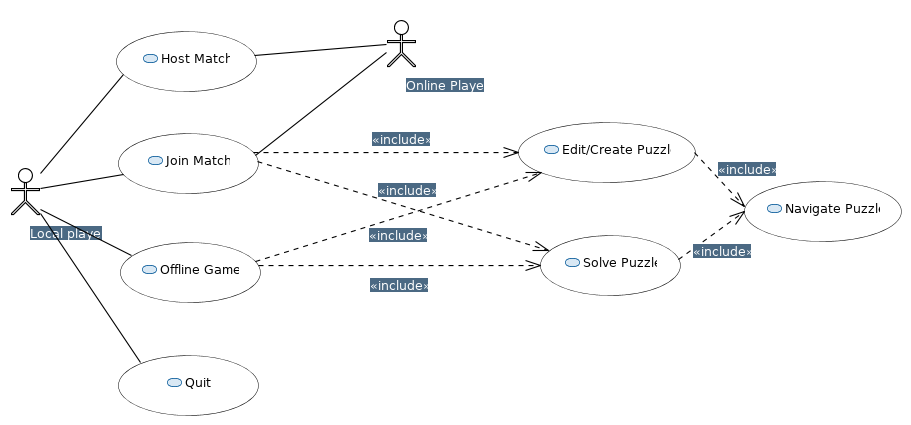
\includegraphics[width=6in]{use_cases.png}
        \caption{Use Case Diagram}
    \end{figure}

\subsection{Actor Descriptions}
    \begin{description}
        \item[Local player] is the local user and has full
            access to the mouse and keyboard or touchscreen interface.
        \item[Online player] is a nonlocal player. There is two-way
            communication between this type of player and the local player.
            There may be 0 or more online players.
        \item[The Host] has special powers, may disconnect other players and
            block players from selecting different puzzles. This player could
            be Local or Online.
    \end{description}

\subsection{Use-case Descriptions}
\begin{mdframed}
    \subsubsection{Host match}
    \begin{description}
        \item[Entry conditions] Internet connection.
        \item[Exit conditions] Will return to game menu. All players
            disconnected or all puzzled have been solved.
        \item[Participating Actors] Online player and local player.
        \item[Flow of events]:
            \begin{enumerate}
                \item The user presses the appropriate menu button.
                \item User creates a game, selects number of players and game
                    type
                \item User shares (friendly looking) match ID with other
                    players. These players may connect to the match
                \item Puzzle Selector appears.
                \item The user may configure the game with this screen.
                    This
                    entails choosing a puzzle and a game mode (edit or solve).
                    Other players can be prevented from making such
                    modifications.
                \item This Puzzle Selector will create a Puzzle Scene
                \item The scene will change from the main menu to the Puzzle
                    Scene.
                \item Additional viewports will be added. These show the
                    progress of online players.

            \end{enumerate}
    \end{description}
\end{mdframed}

\begin{mdframed}
    \subsubsection{Join match}
    \begin{description}
        \item[Entry conditions] Internet connection. The menu must be present.
        \item[Exit conditions]
        \item[Exit conditions] Will return to game menu. All players
            disconnected or all puzzled have been solved.
        \item[Participating Actors] Online player and local player.
        \item[Flow of events]:
            \begin{enumerate}
                \item The user presses the appropriate menu button.
                \item Puzzle Selector appears.
                \item The user may configure the game with this screen, if
                    the game host allows it. This would
                    entail choosing a puzzle and a game mode (edit or solve).
                \item This Puzzle Selector will create a Puzzle Scene
                \item The scene will change from the main menu to the Puzzle
                    Scene.
                \item Additional viewports will be added. These show the
                    progress of online players.
            \end{enumerate}
    \end{description}
\end{mdframed}


\begin{mdframed}
    \subsubsection{Offline game}
    \begin{description}
        \item[Entry conditions] Menu must be present.
        \item[Exit conditions] Will return to game menu. Puzzle has been
            solved.
        \item[Participating Actors] Local player.
        \item[Flow of events]:
            \begin{enumerate}
                \item User selects the appropriate menu button.
                \item Puzzle Selector appears.
                \item The user may configure the game with this screen. This
                    entails choosing a puzzle and a game mode (edit or solve).
                \item This Puzzle Selector will create a Puzzle Scene
                \item The scene will change from the main menu to the Puzzle
                    Scene.
            \end{enumerate}
    \end{description}
\end{mdframed}


\begin{mdframed}
    This use case includes the Host Match, Join Match and Offline Game
    use cases.
    \subsubsection{Edit puzzle}
    \begin{description}
        \item[Entry conditions] A Puzzle Scene must be loaded and edit mode
            must be activated.
        \item[Exit conditions] Will return to game menu. The puzzle may be
            saved to the disk.
        \item[Participating Actors] Online player or local player.
        \item[Flow of events]:
            \begin{enumerate}
                \item The user navigates the puzzle
                \item If a position on the grid is selected, the Block Modifier
                    is presented. This position may be empty or it may
                    contain a block.
                \item The user may change properties of the block using this
                    screen.
                \item Blocks may be added or removed using this same screen.
            \end{enumerate}
            Puzzle preview:
            \begin{enumerate}
                \item User may press the preview button
                \item The user will try the puzzle in Solve Puzzle mode until
                    that mode's exit conditions are met.
                    A special banner will graphically indicate preview mode.
                \item The solving scene will have a special button for
                    returning to the editing scene
            \end{enumerate}
    \end{description}
\end{mdframed}


\begin{mdframed}
    This use case includes the Host Match, Join Match and Offline Game
    use cases.
    \subsubsection{Solve puzzle}
    \begin{description}
        \item[Entry conditions] A Puzzle Scene must be loaded and solve mode
            must be activated.
        \item[Exit conditions] Will return to game menu or puzzle editor.
            If the game is over, an overview of results will be shown and the
            steps taken to solve the puzzle may be saved to the disk.
        \item[Participating Actors] Online player or local player.
        \item[Flow of events]:
            \begin{enumerate}
                \item The user navigates the puzzle
                \item If a block is selected, the block runs any associated
                    Block Action.
                \item These Block Actions may modify the block's properties or
                    request the addition or removal of blocks, including the
                    selected block, from the Grid Manager.
                \item This sequence is repeated until the winning block is
                    found, the user quits, or a losing condition is met.
                \item User's actions may be mirrored on an online player's
                    screen, likewise, separate Puzzle Scenes  may be updated
                    with any moves made by other players.
            \end{enumerate}
    \end{description}
\end{mdframed}


\begin{mdframed}
    \subsubsection{Navigate puzzle}
    This use case includes the Solve puzzle and Edit puzzle use cases.
    \begin{description}
        \item[Entry conditions] Puzzle scene loaded and permission to move.
            Input devices must be functional.
        \item[Exit conditions] The game must offer continuous feedback.
            If the entry conditions are met, any further input must be
            acted on as soon as possible.
        \item[Participating Actors] Online player and local player.
        \item[Flow of events]:
            Camera motion.
            \begin{enumerate}
                \item User drags with a mouse or touchscreen
                \item The camera changes position
            \end{enumerate}

            Block selection.
            \begin{enumerate}
                \item User clicks with mouse or taps on touchscreen
                \item The 3D coordinates are translated into a position on
                    a game ``board.''
                \item The Grid Manager is notified of input and the grid
                    position.
                \item If a block is present there, it is selected and activated.
                    Exact actions depend on the game mode.
                \item If a block is not present, the space is selected. This
                    is only useful in edit mode.
                \item The user may end the game at any point through the pause
                    menu.
            \end{enumerate}

    \end{description}
\end{mdframed}


\begin{mdframed}
    \subsubsection{Quit}
    \begin{description}
        \item[Entry conditions] Game must be running. This action is
            asynchronous and may activate at any point.
        \item[Exit conditions] Game, be gone!
        \item[Participating Actors] Local player.
        \item[Flow of events]:
            \begin{enumerate}
                \item User presses the quit button on a menu
                \item or User presses appropriate sequence of keys, such as
                    the escape key or the alt and F4 combo.
                \item The program shuts down gracefully.
            \end{enumerate}
    \end{description}
\end{mdframed}



% reqs analysis
\section{Requirements Analysis}

\subsection{Structural Analysis}\label{struct-analysis-BC}
% Briefly describe each analysis class (organized according to type - boundary,
% control, and entity) and class diagrams

\subsection{Behavioral Analysis}\label{behavioral-analysis-HR}

Each use case has been realized using a sequence diagram. In addition, an
activity diagram has been prepared in order to demonstrate the creation of a
Puzzle instance by the Local Player.
% Puzzles instantiated in either edit or solve mode, maybe progress is shared
% with opponents. Players interact through the navigate puzzle use-case,
% can exit game during puzzle or goto menu or stay until solved, then go to
% scoreboard
    \begin{figure}[H]
        \centering
        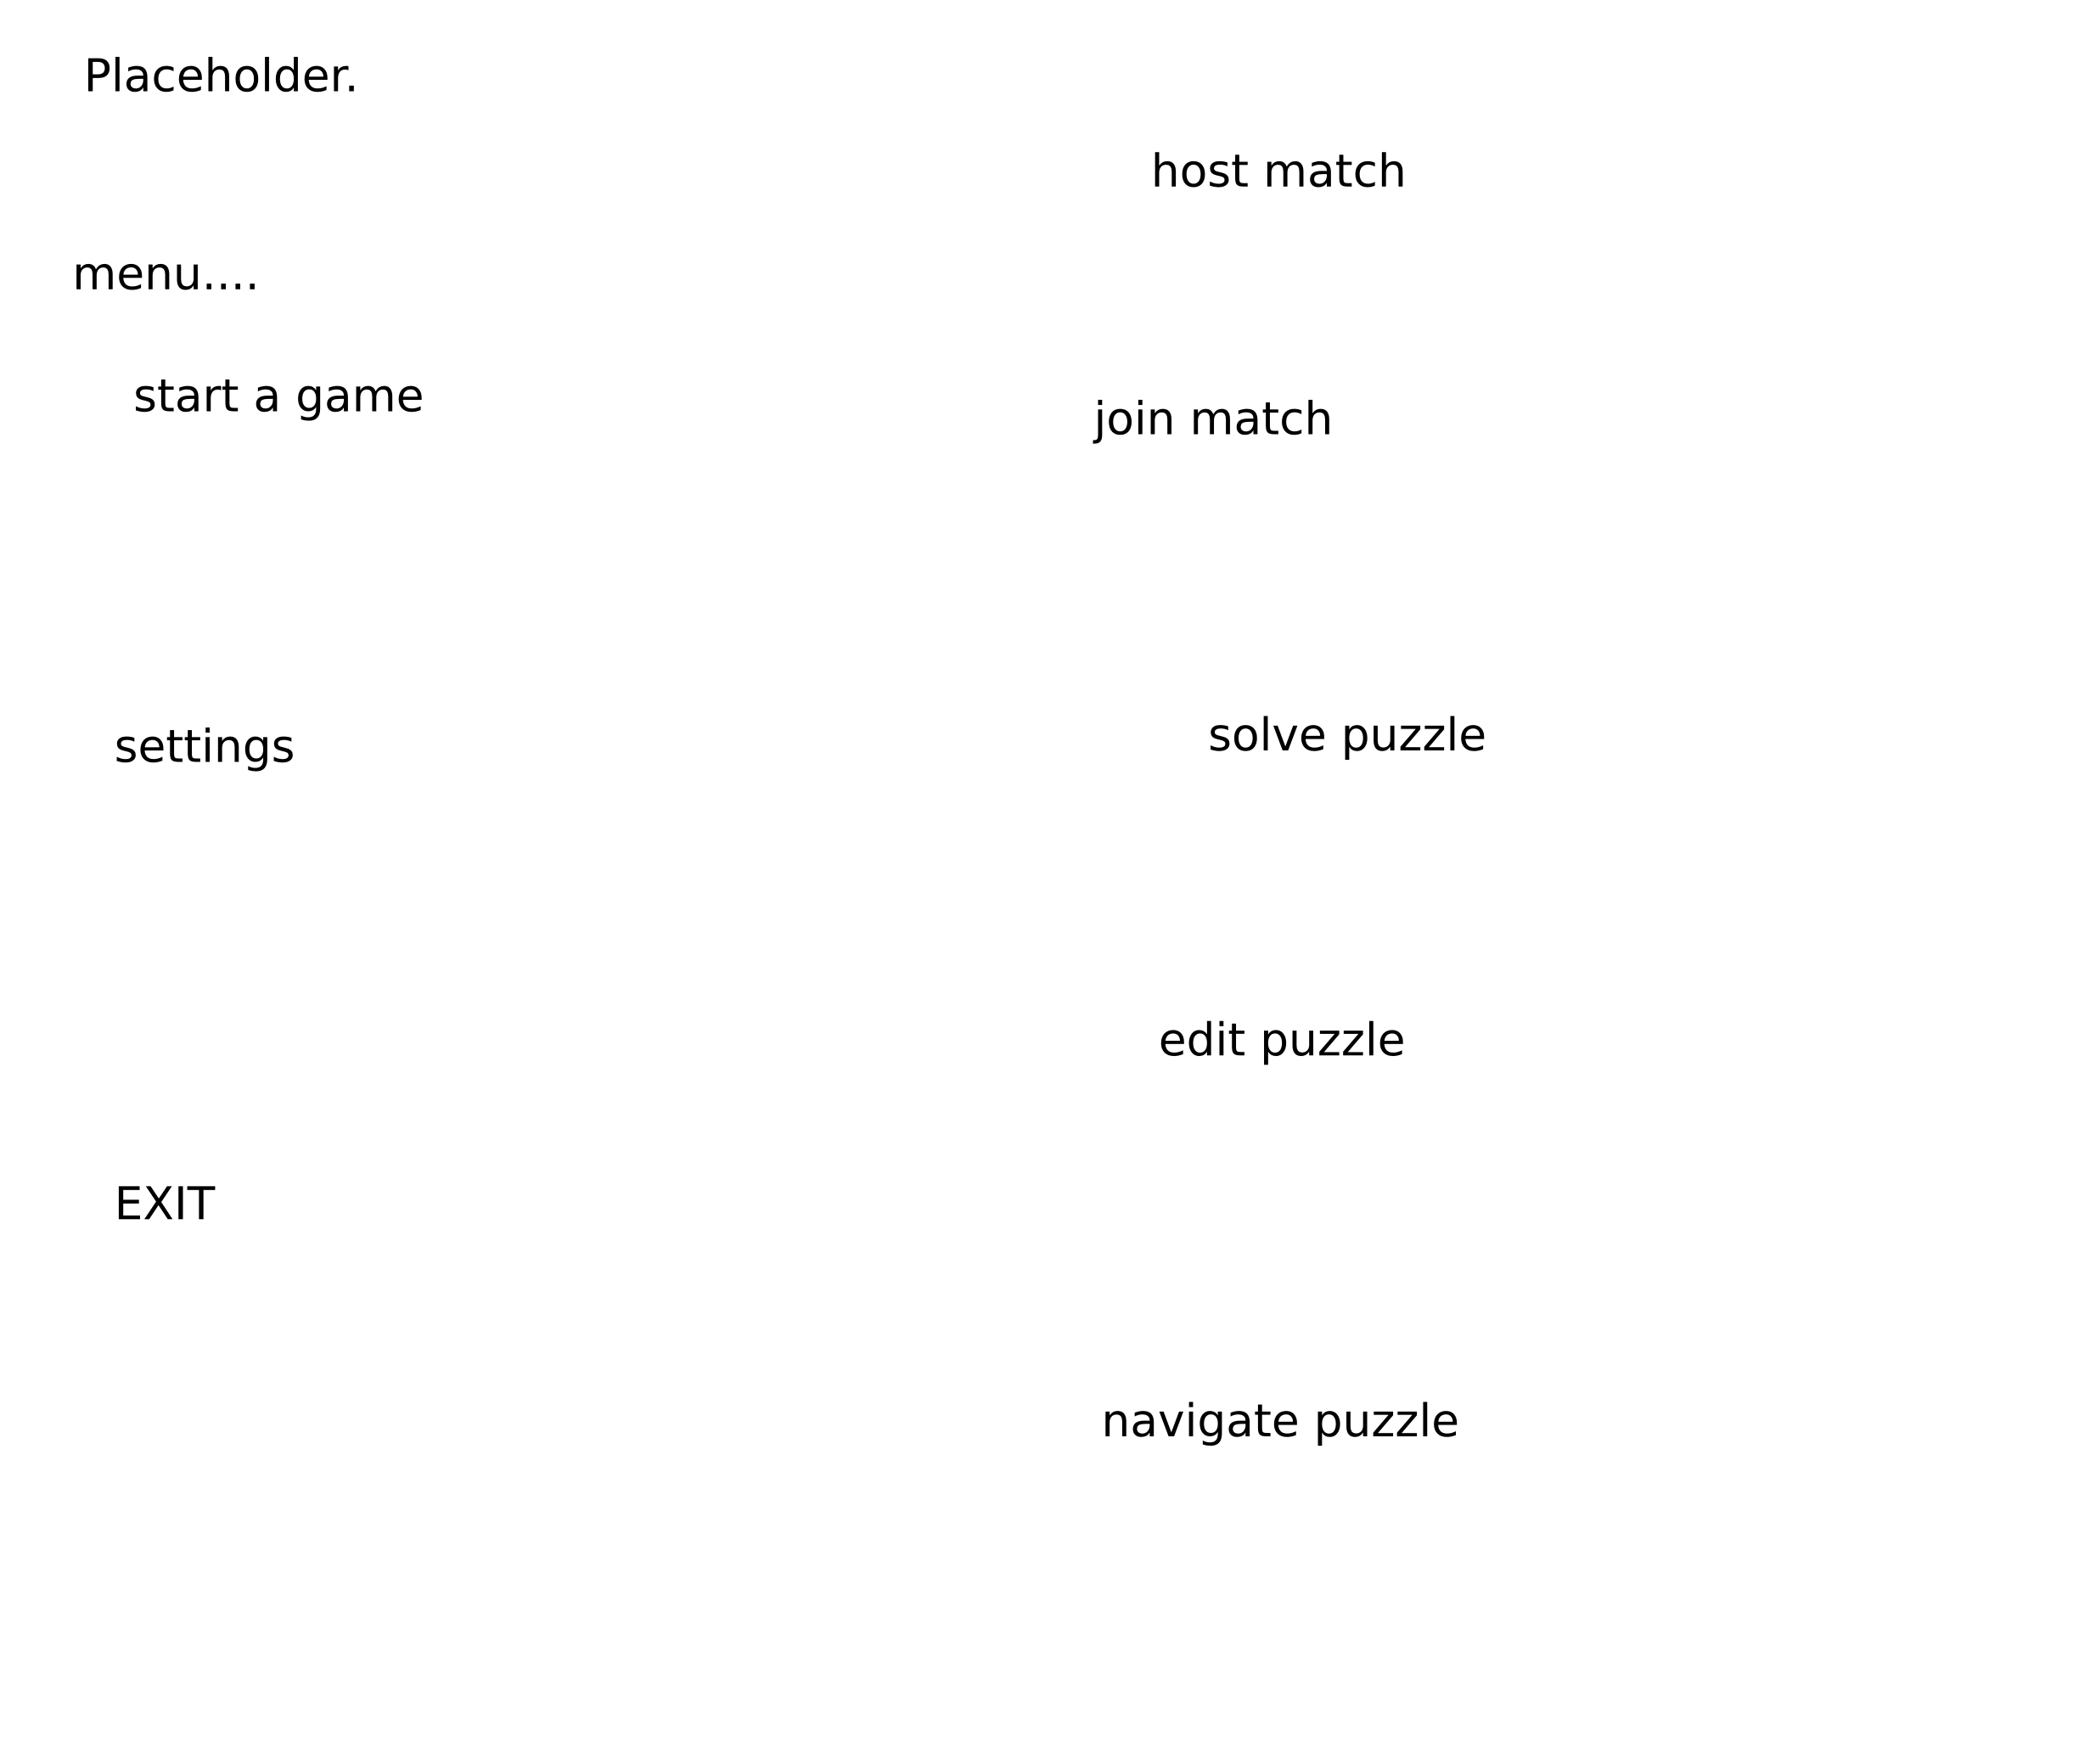
\includegraphics[width=3in]{activity_all.png}
        \caption{Puzzle instantiation logic represented by a UML Activity Diagram}
    \end{figure}


% should've used \forloop
    \begin{figure}[H]
        \centering
        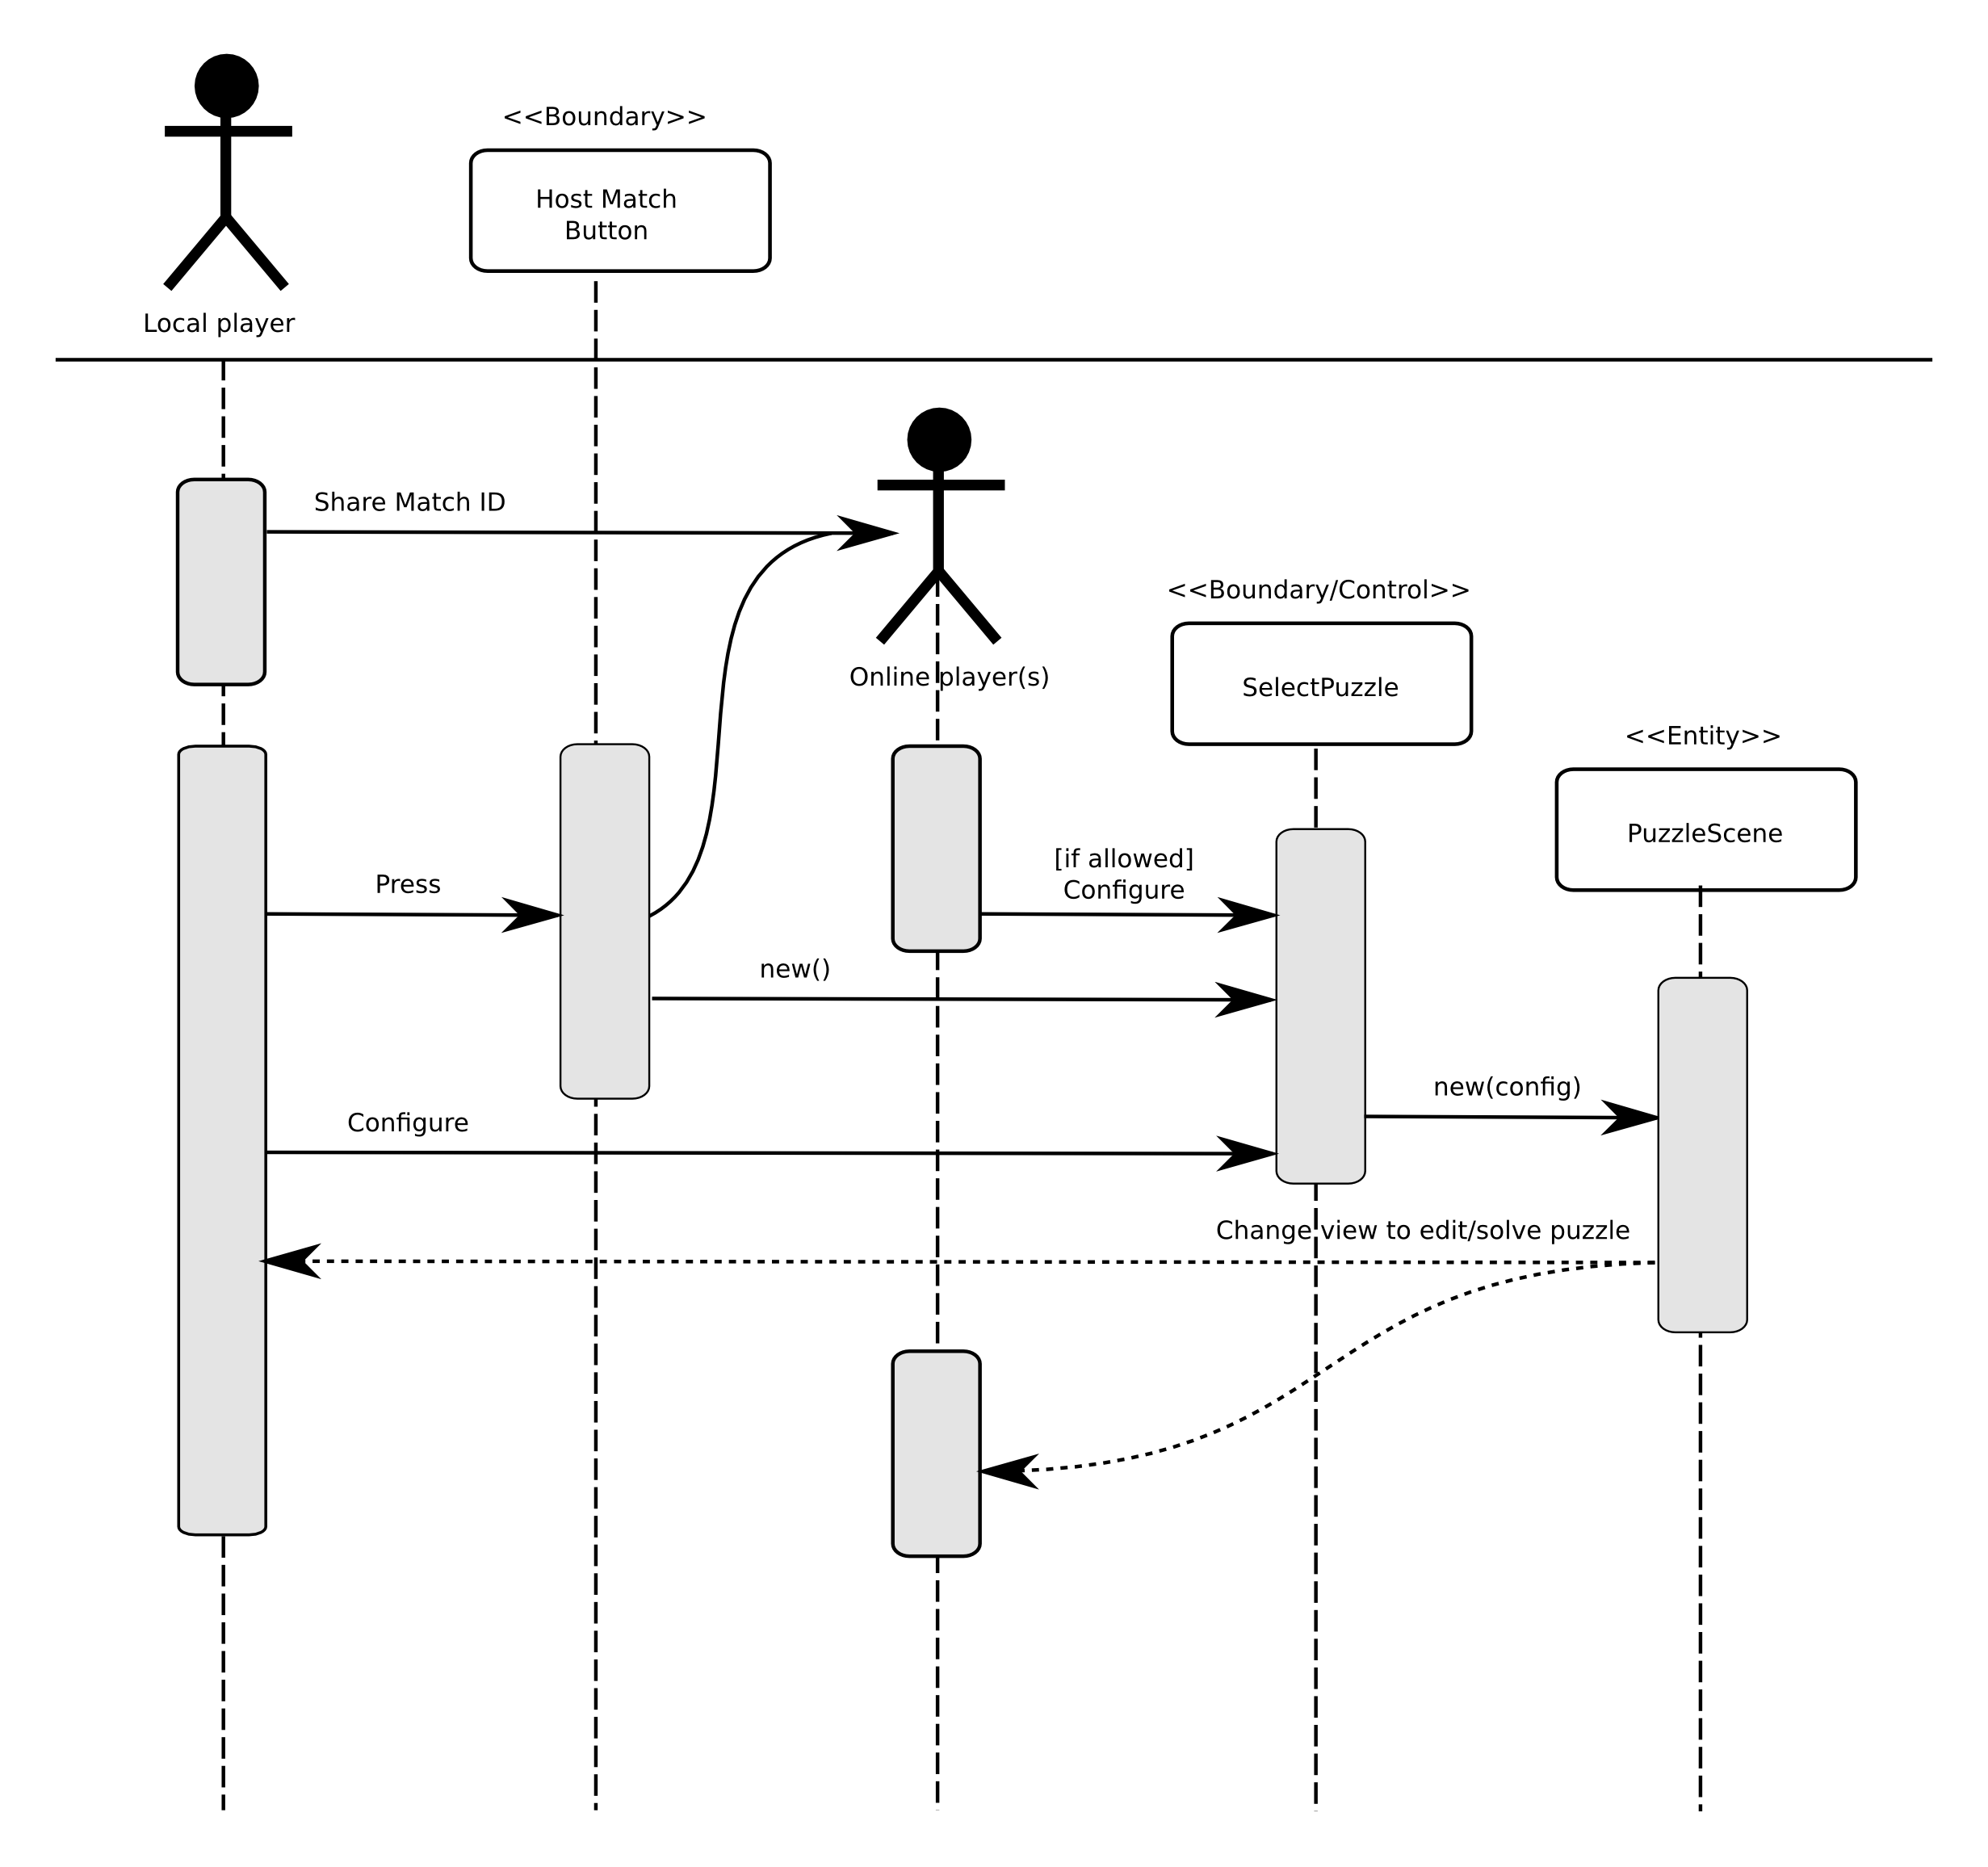
\includegraphics[width=4.5in]{sequence_host_match.png}
        \caption{UML Sequence Diagram for hosting a multiplayer game.}
    \end{figure}


    \begin{figure}[H]
        \centering
        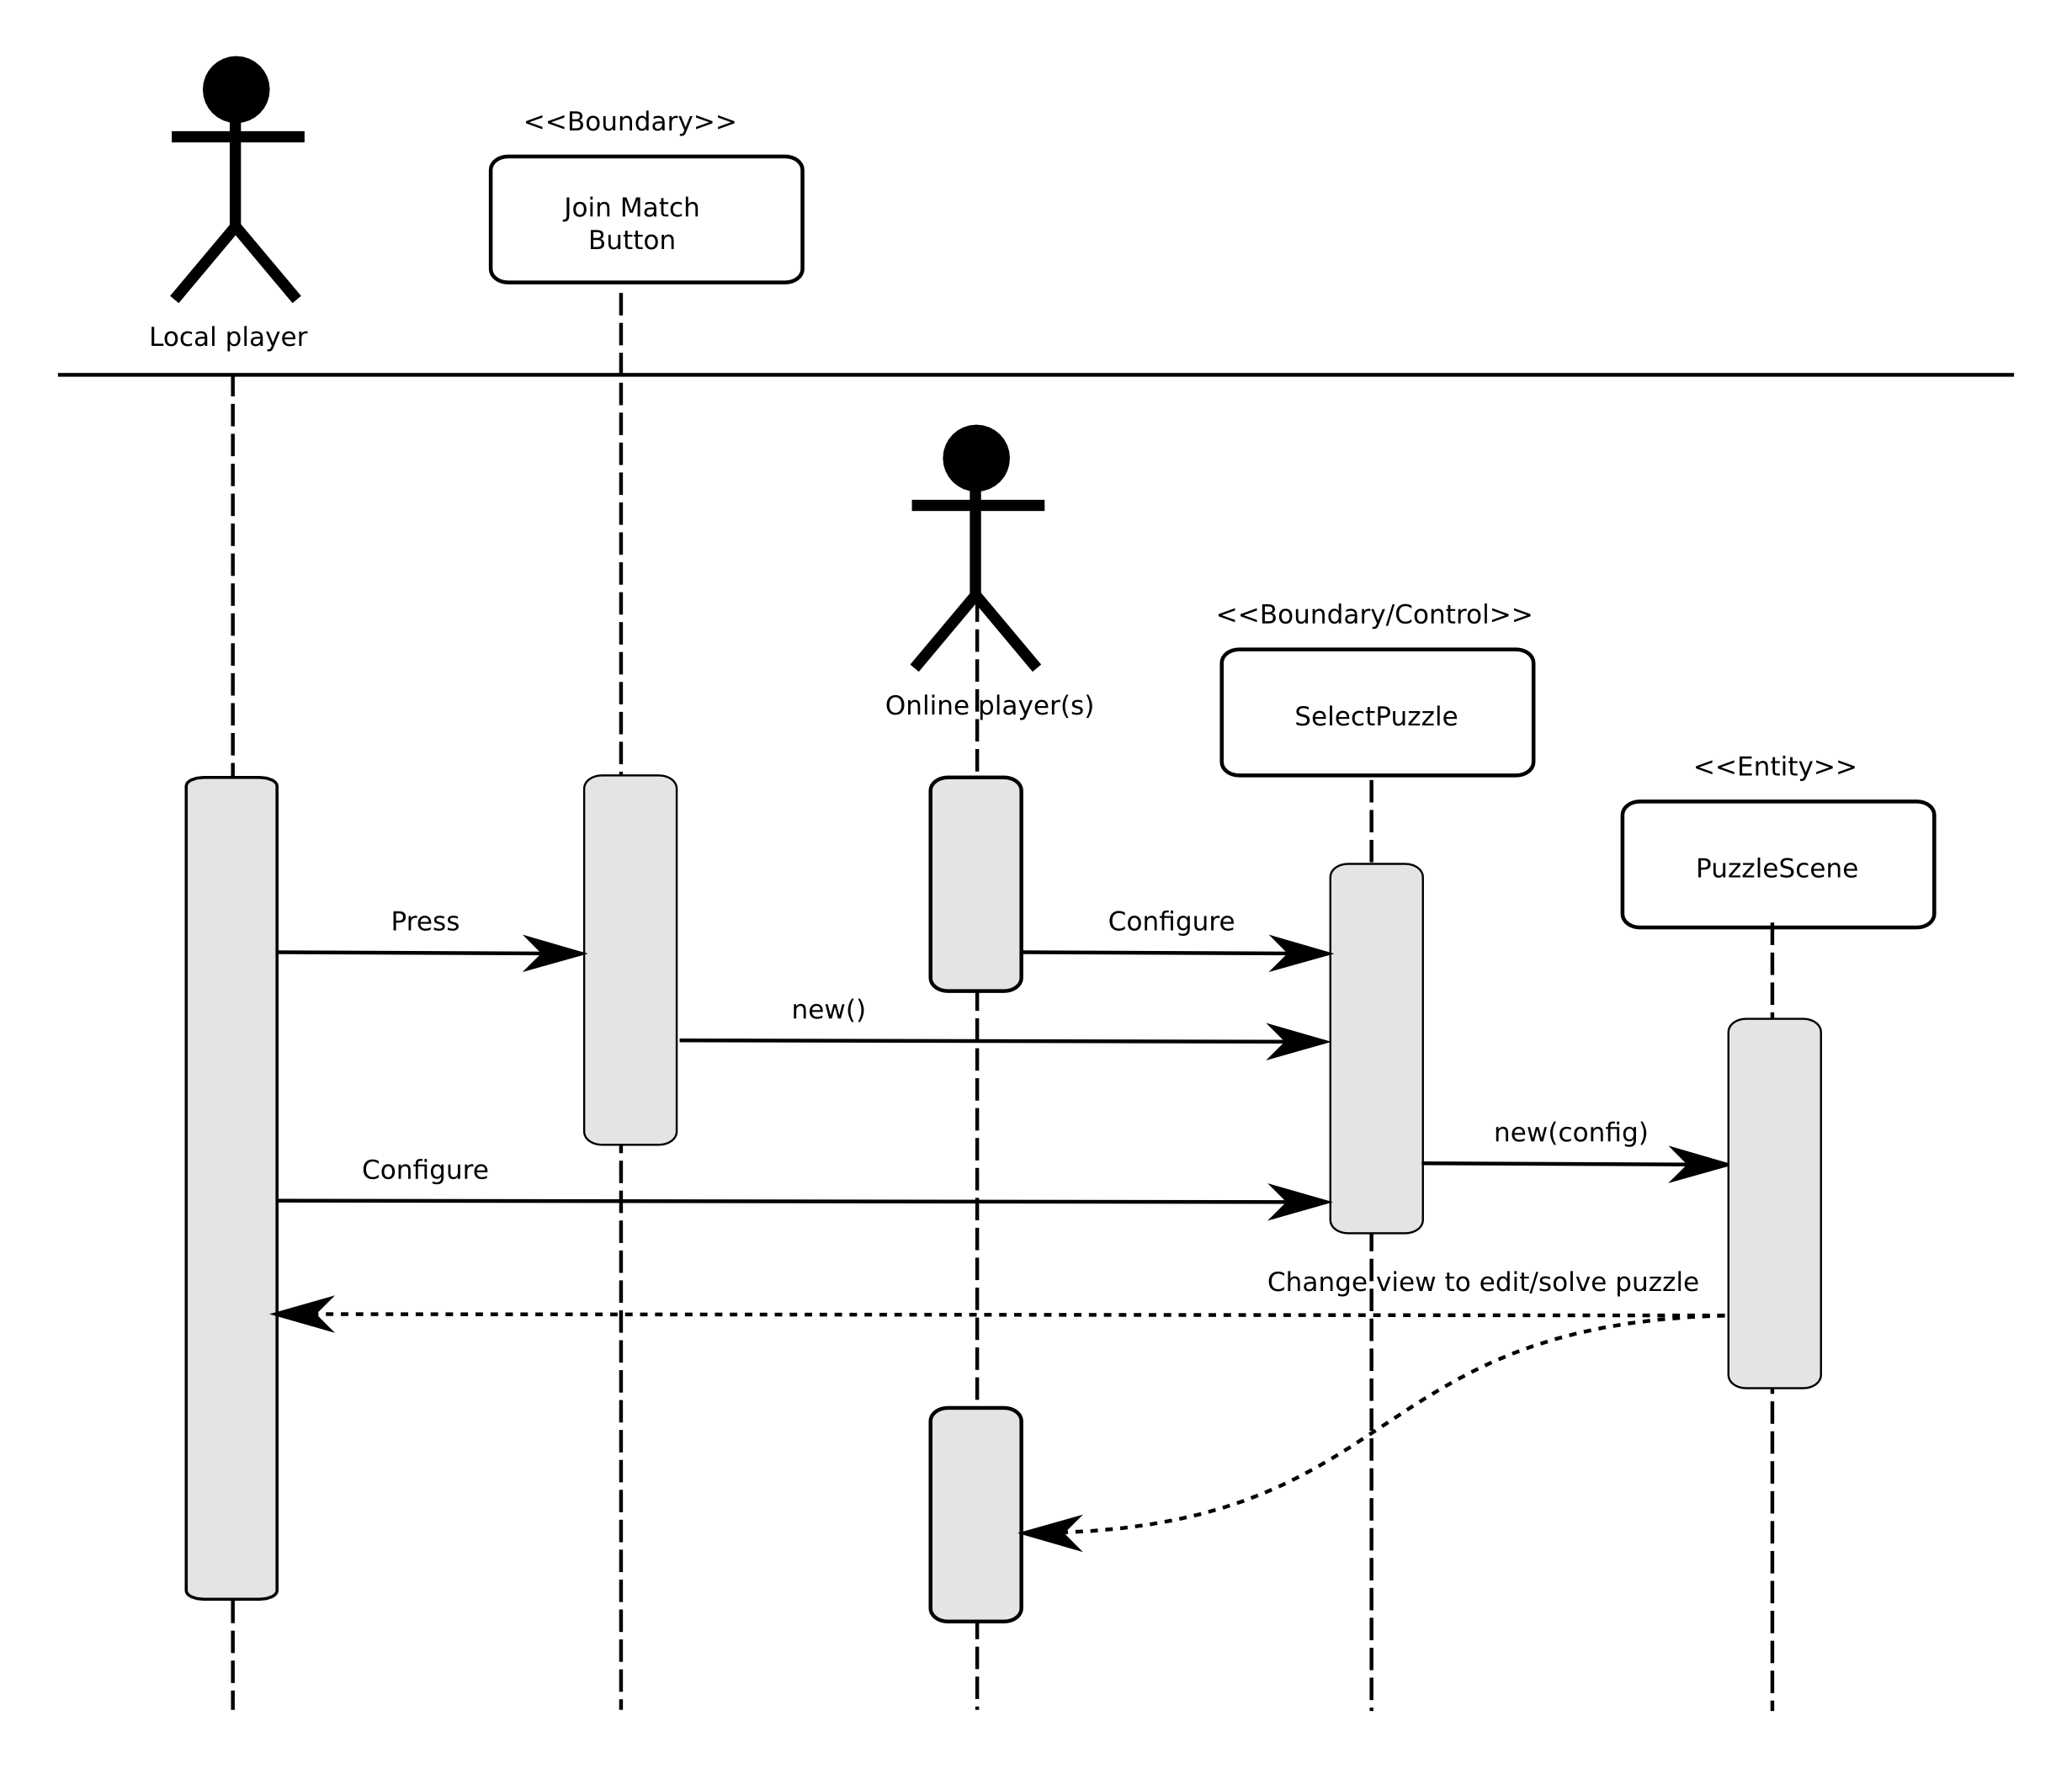
\includegraphics[width=4.5in]{sequence_join_match.png}
        \caption{UML Sequence Diagram for joining a multiplayer game.}
    \end{figure}


    \begin{figure}[H]
        \centering
        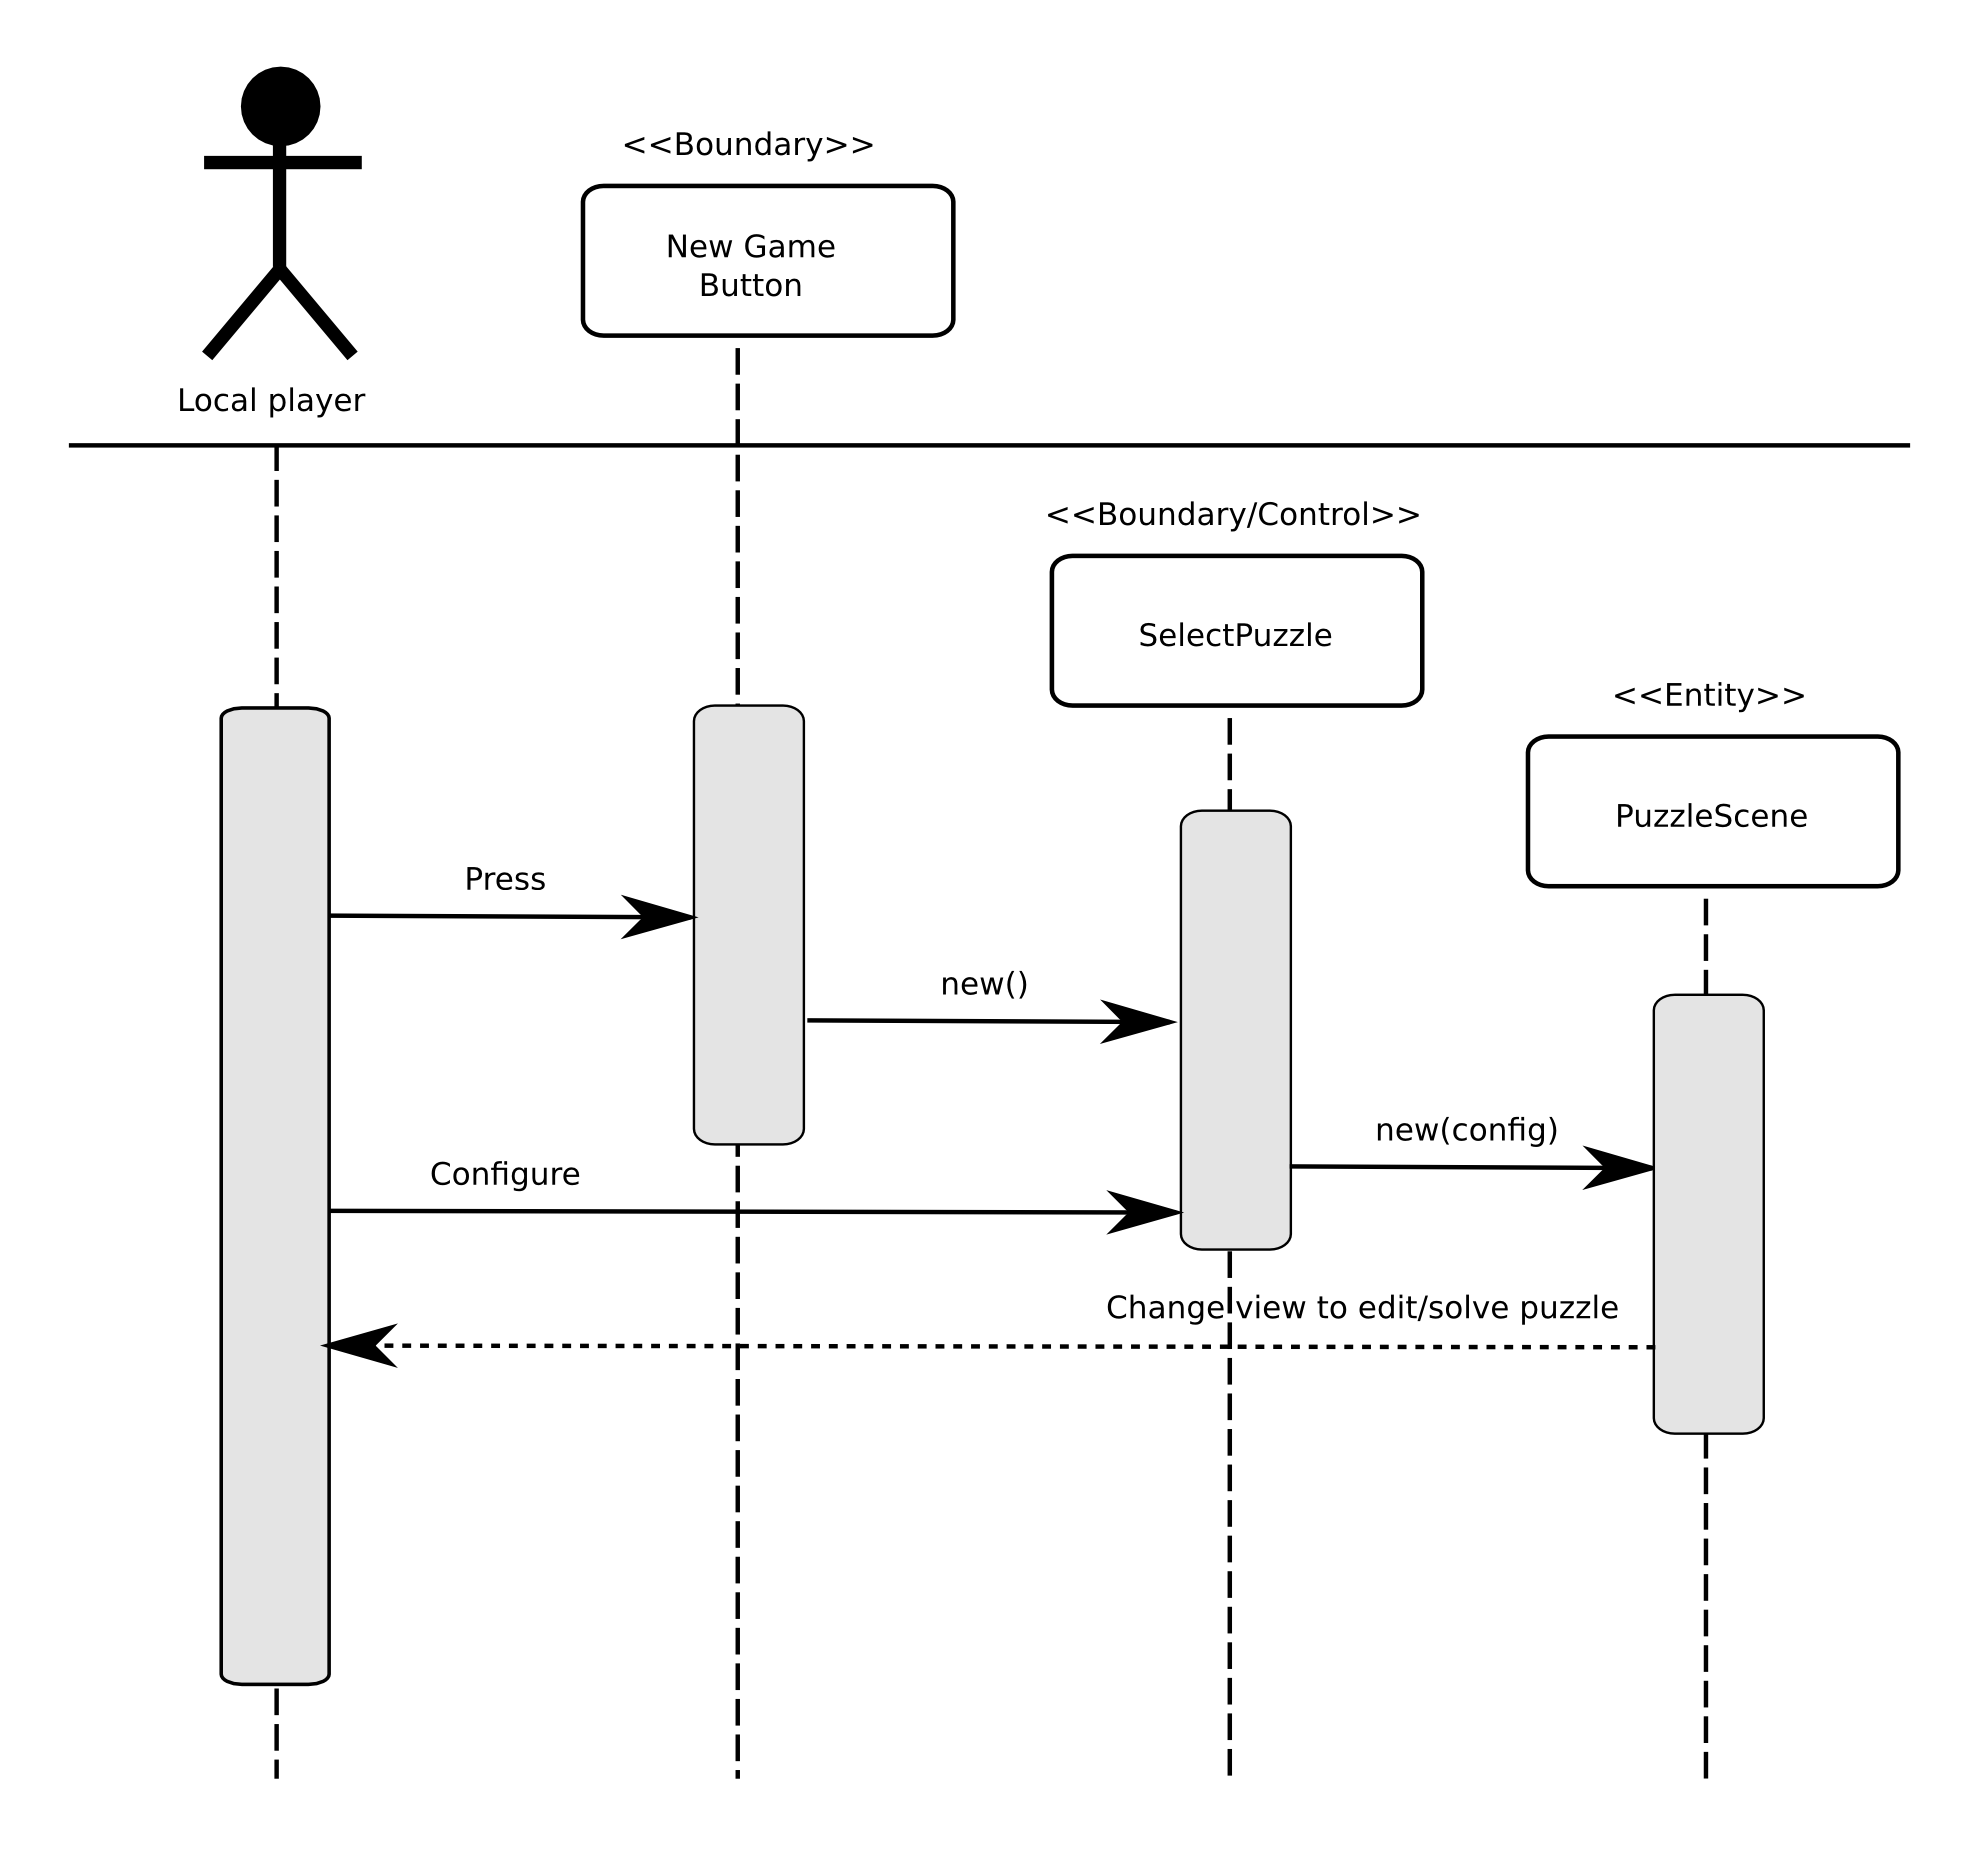
\includegraphics[width=4.5in]{sequence_offline_play.png}
        \caption{UML Sequence Diagram for an offline game.}
    \end{figure}


    \begin{figure}[H]
        \centering
        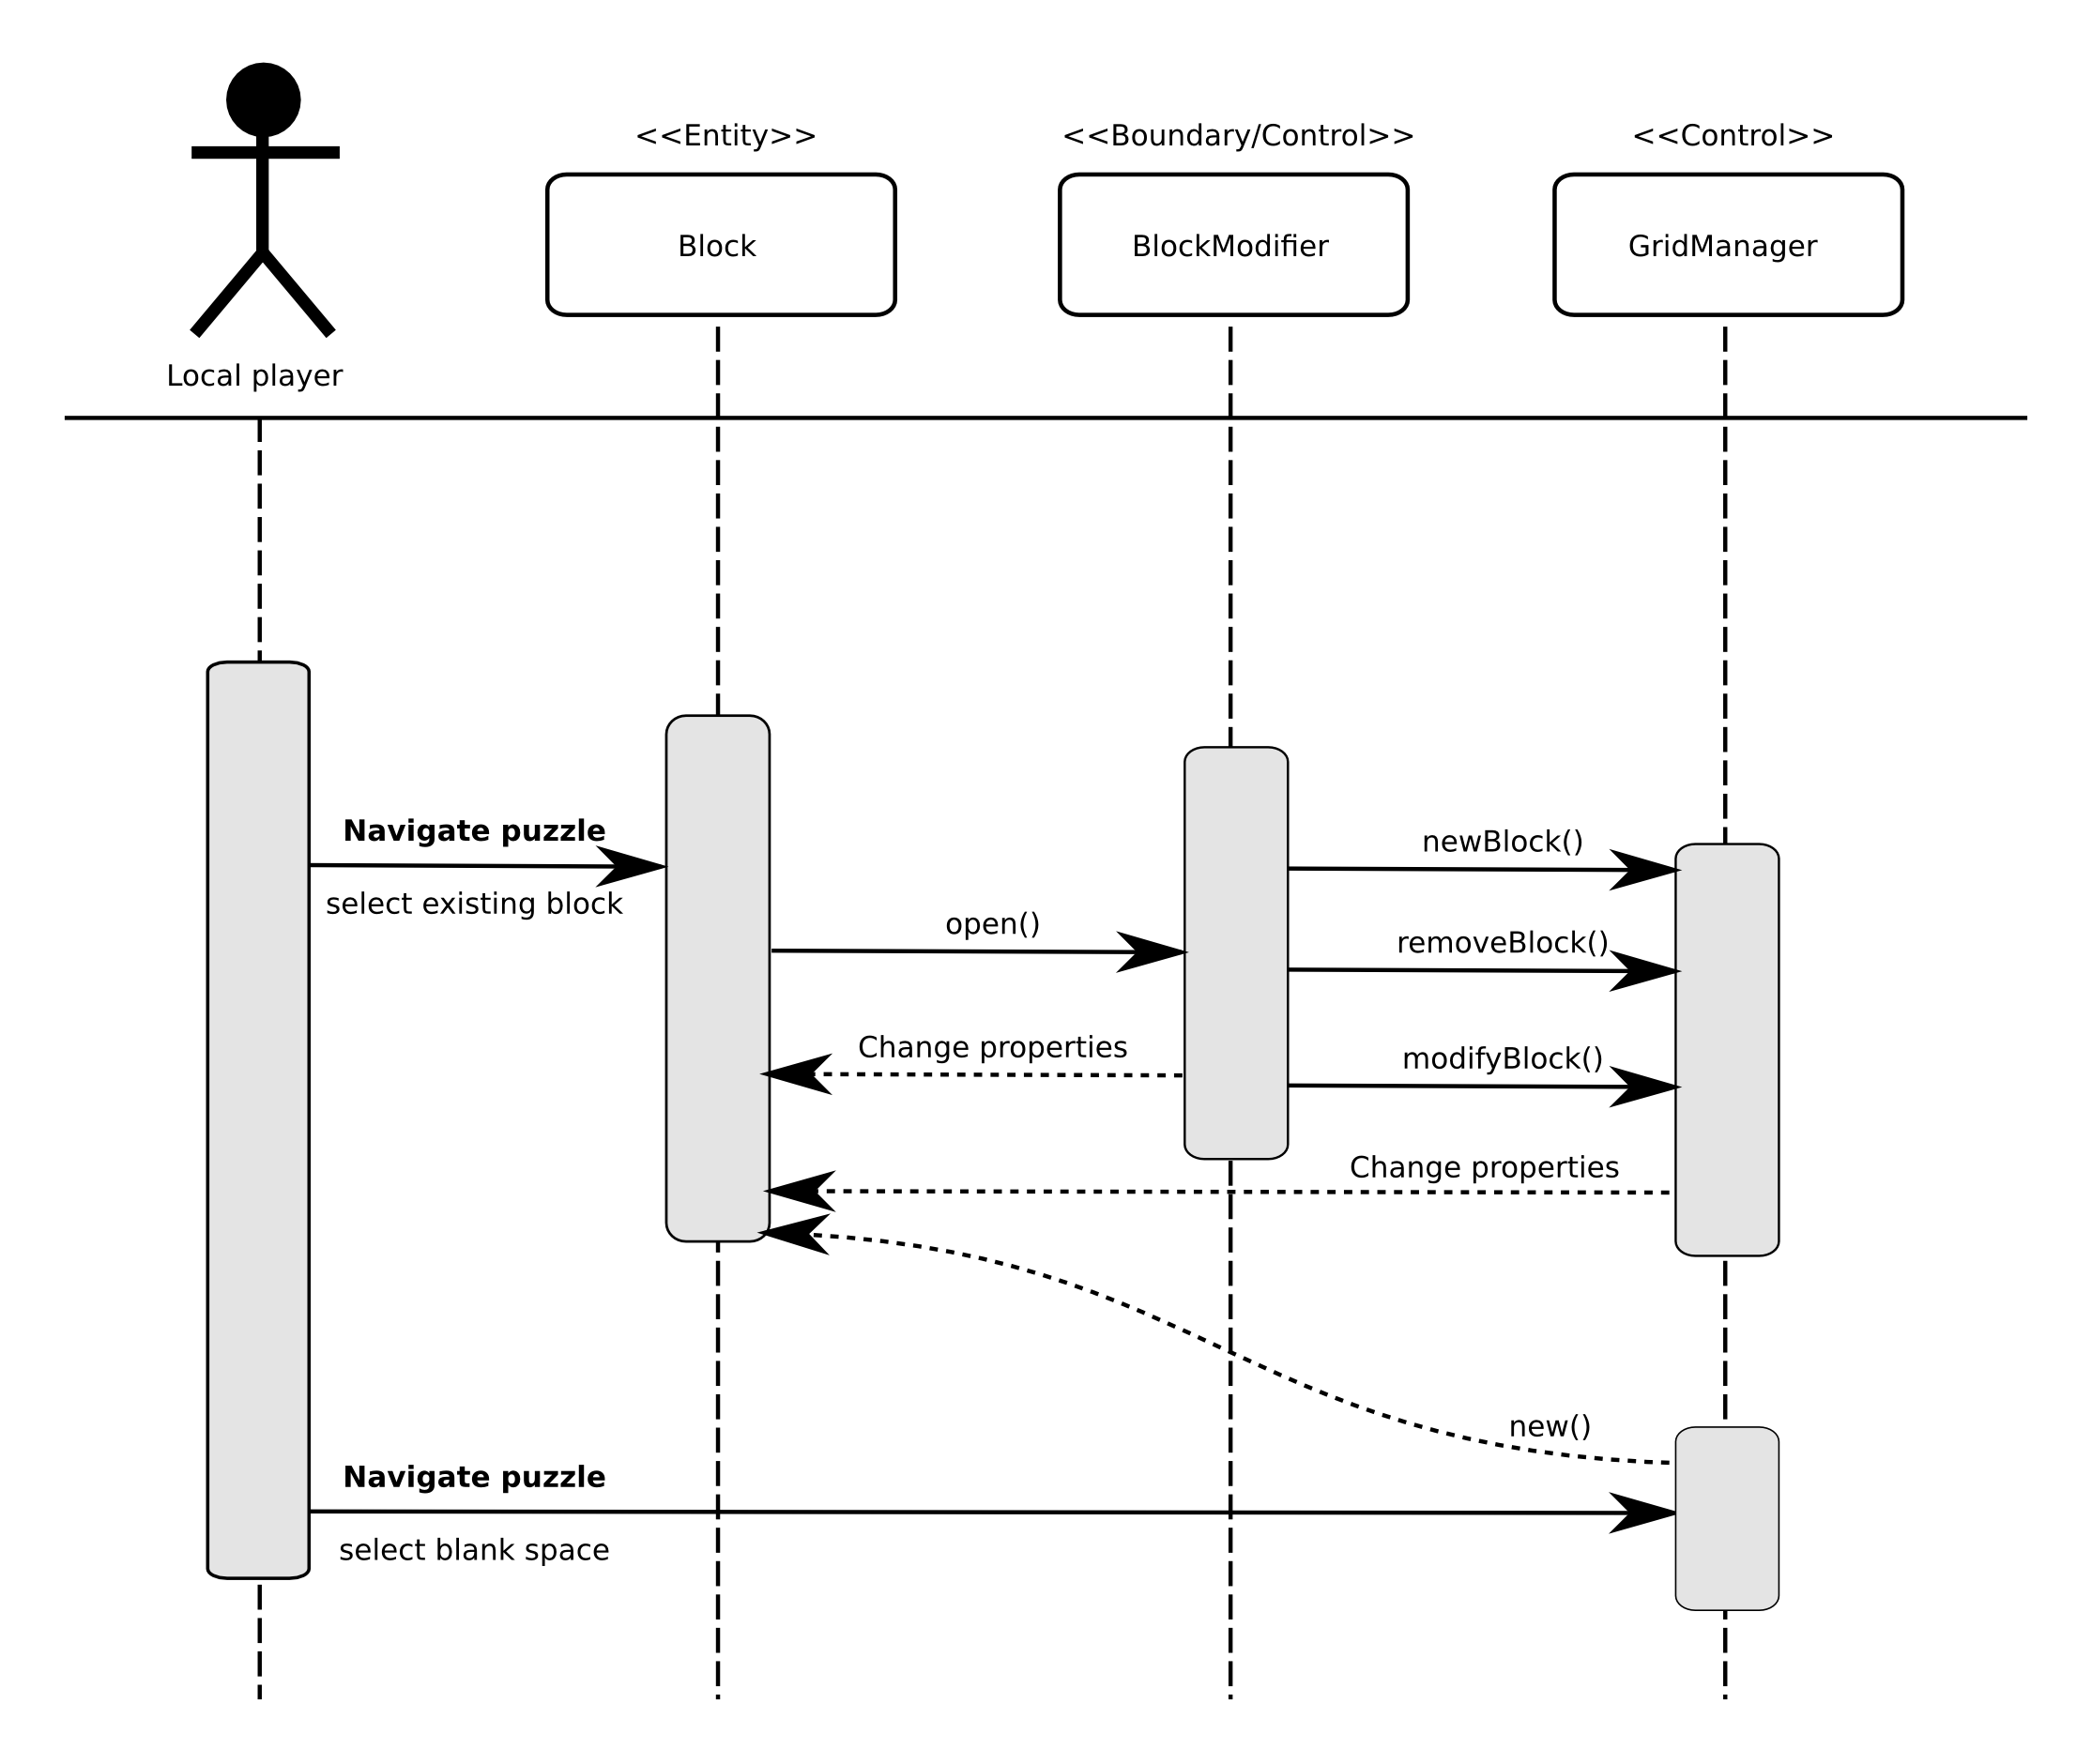
\includegraphics[width=4.5in]{sequence_edit.png}
        \caption{UML Sequence Diagram for editing or creating a puzzle.}
    \end{figure}


    \begin{figure}[H]
        \centering
        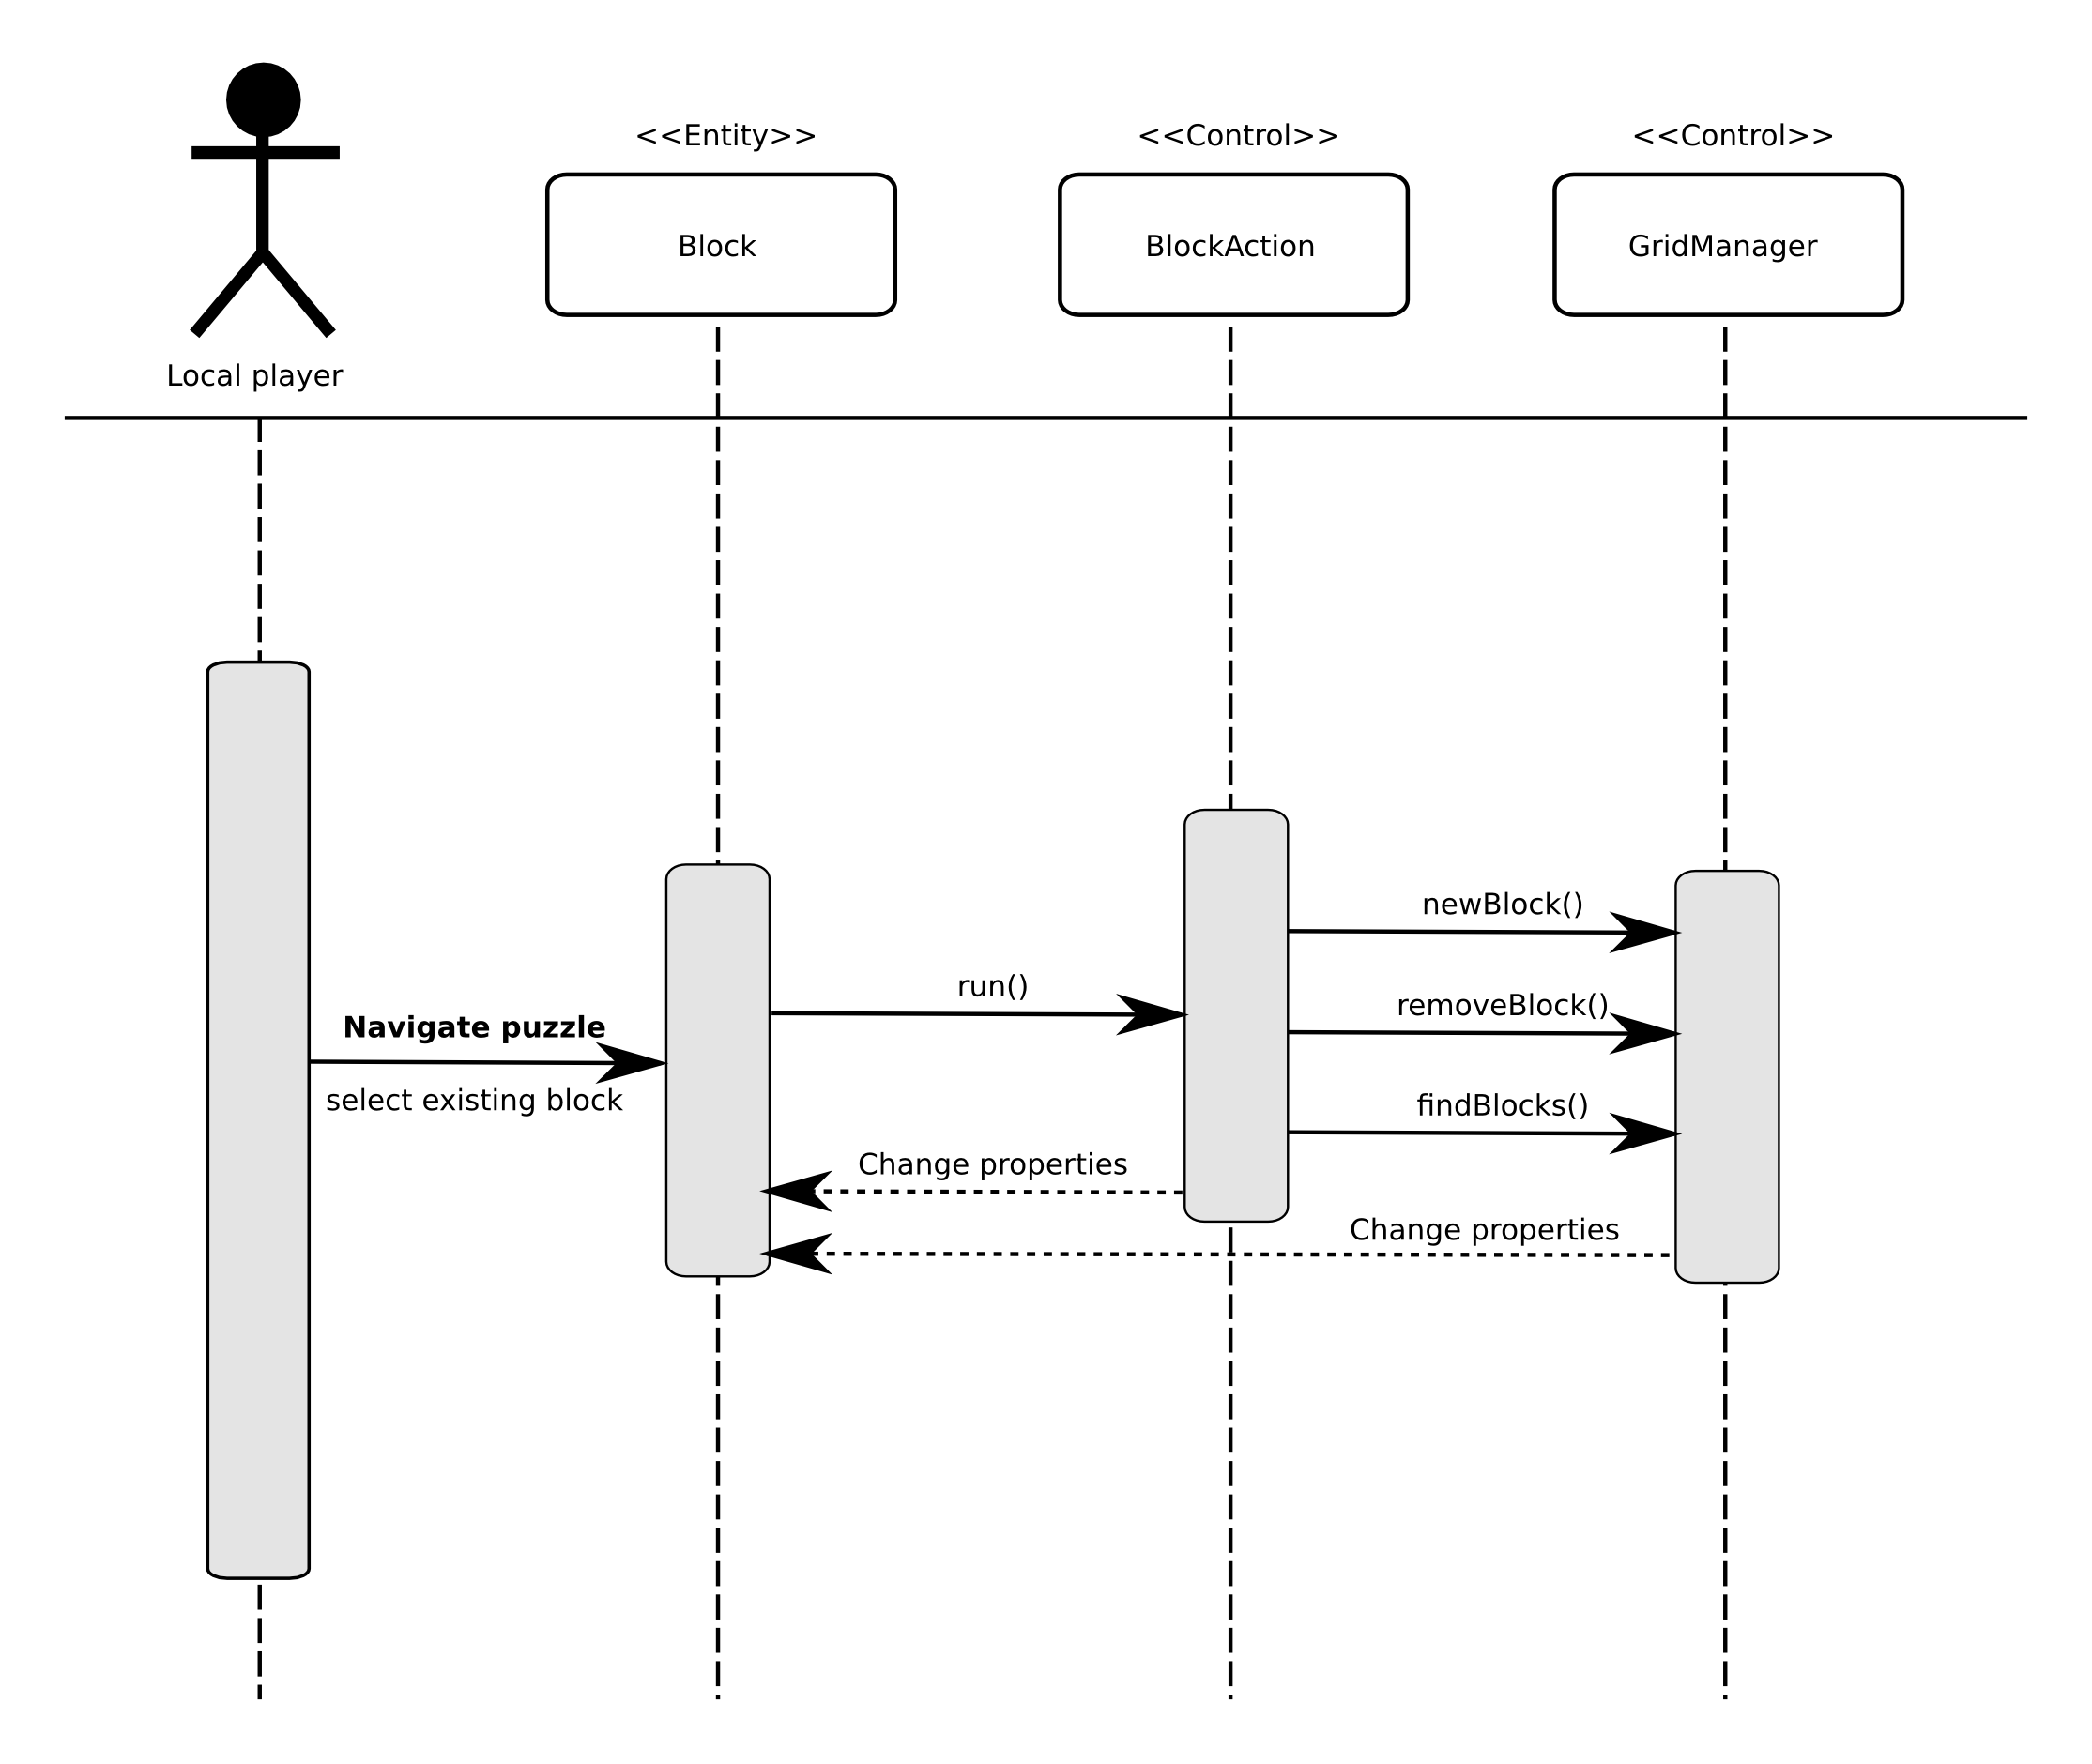
\includegraphics[width=4.5in]{sequence_solve.png}
        \caption{UML Sequence Diagram for the puzzle solving process.}
    \end{figure}


    \begin{figure}[H]
        \centering
        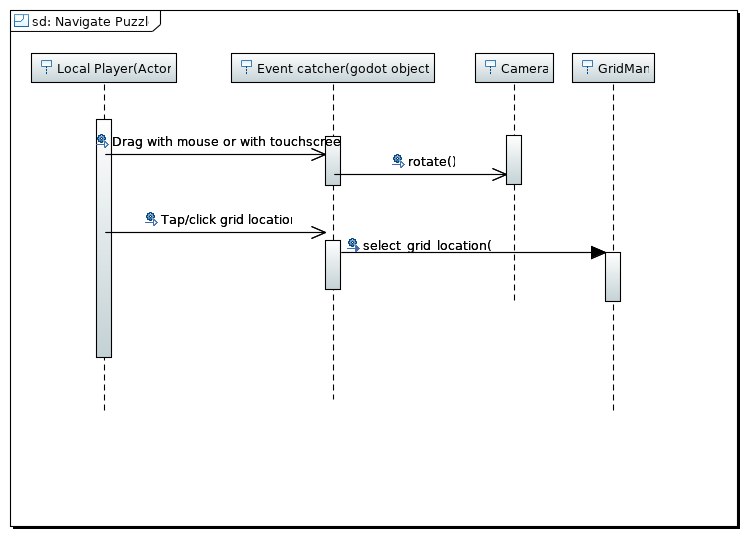
\includegraphics[width=4.5in]{sequence_navigate_puzzle.png}
        \caption{UML Sequence Diagram for navigating a puzzle in either edit or
        solve mode.}
    \end{figure}


    \begin{figure}[H]
        \centering
        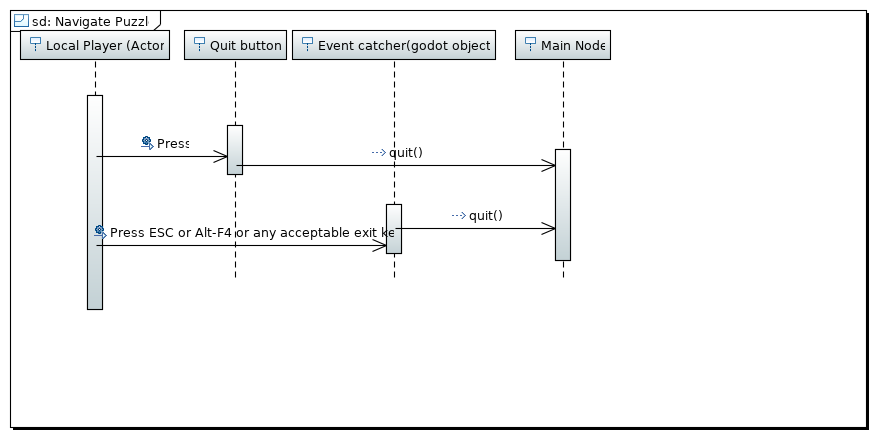
\includegraphics[width=4.5in]{sequence_quit.png}
        \caption{UML Sequence Diagram demonstrating game-shutdown.}
    \end{figure}




\subsection{User Interface Analysis}\label{UI-analysis-CA}
The user interface in Anttris will follow the design of most simple game interfaces. It will include a main menu, configuration menu, play menu, editor interface and game interface. All of these will be connected to each other through the use of buttons on the screen that can be pressed with a mouse, a finger on a touch device and perhaps, with enough time, a game controller. Included below are flow diagrams for the user interface as well as initial design ideas for each individual interface.\\

    \begin{figure}[H]
        \centering
        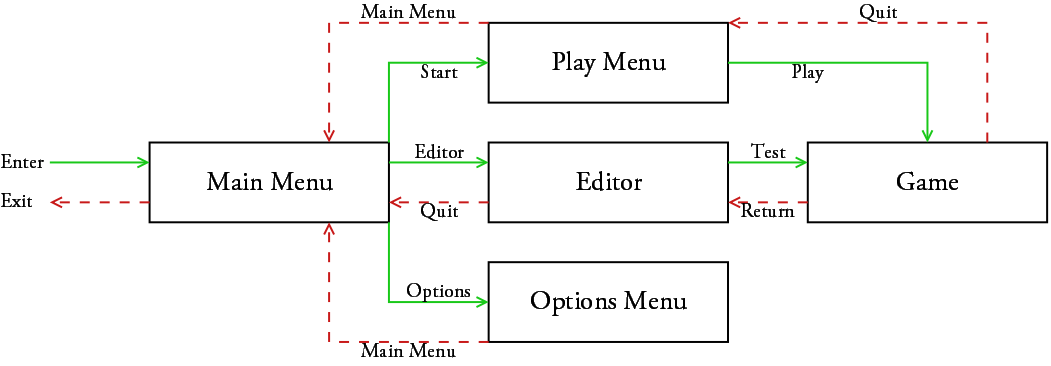
\includegraphics[width=4in]{UIFlow.png}
        \caption{Flow Diagram for UI.}
    \end{figure}
    \begin{figure}[H]
        \centering
        
\includegraphics[width=4in]{MainMenu.png}
        \caption{Main Menu UI. This leads to the Play Menu UI, Editor UI and Option Menu. Exit leaves the program.}
    \end{figure}
    \begin{figure}[H]
        \centering
        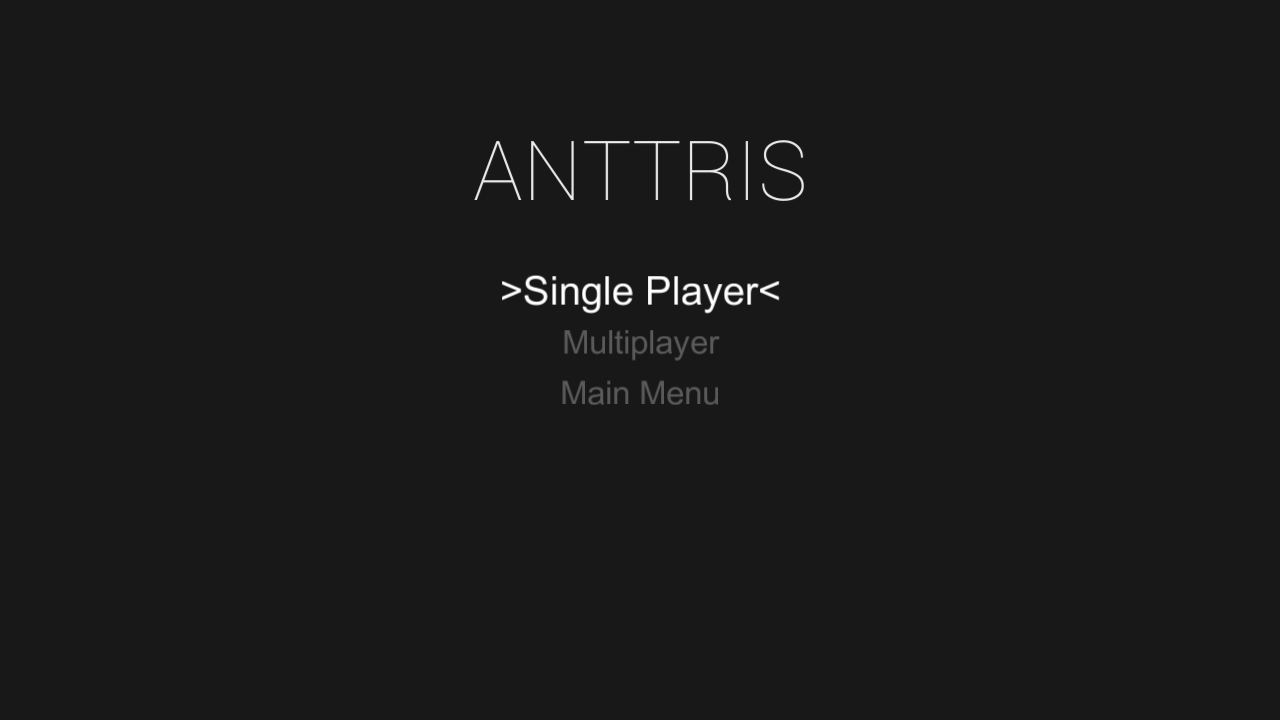
\includegraphics[width=4in]{PlayMenu.png}
        \caption{Play Menu UI. This leads to the Game UI, or back to the Main Menu.}
    \end{figure}
    \begin{figure}[H]
        \centering
        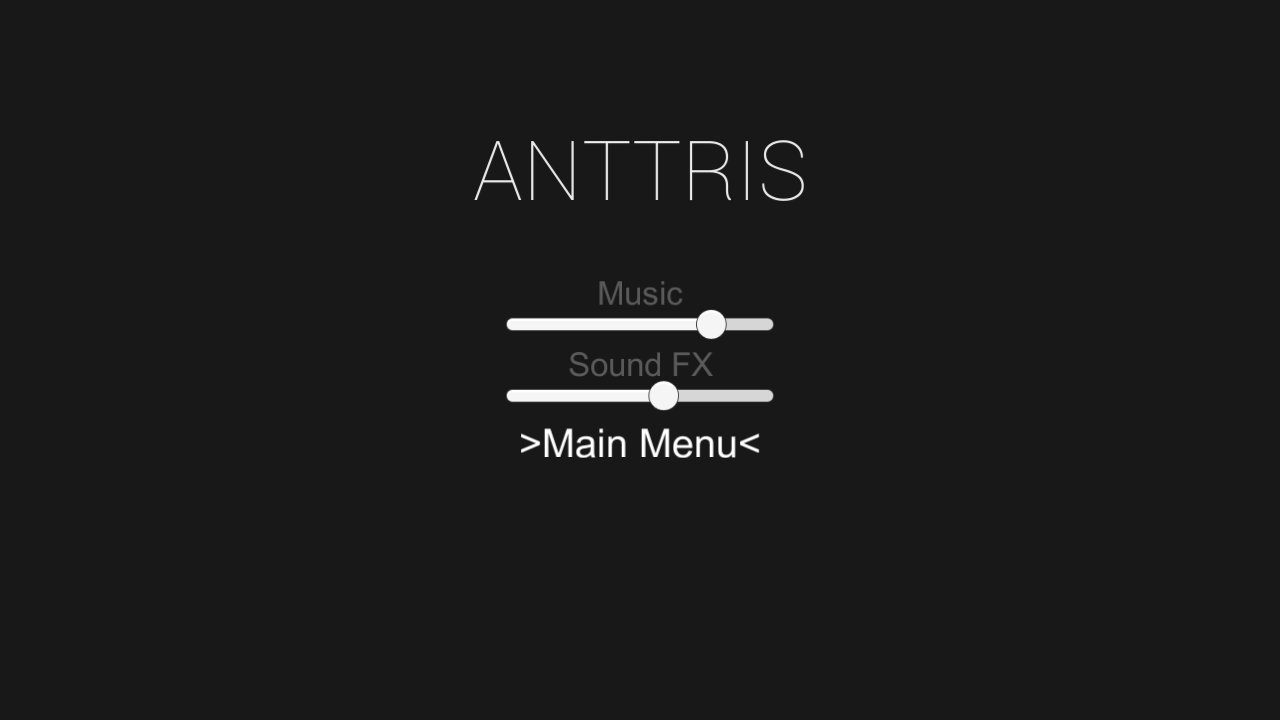
\includegraphics[width=4in]{OptionsMenu.png}
        \caption{Options Menu UI. This leads back to the Main Menu. Options are examples. More options are likely as the game evolves.}
    \end{figure}
	\begin{figure}[H]
        \centering
        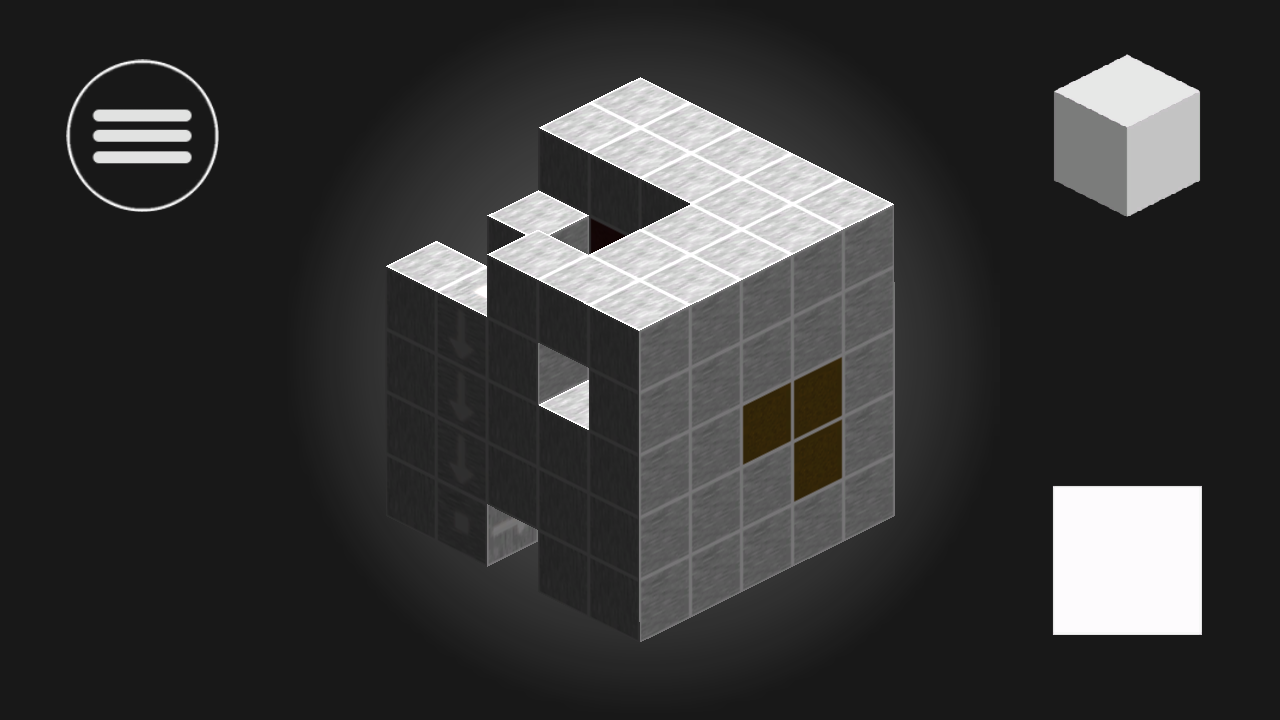
\includegraphics[width=4in]{GameUI.png}
        \caption{Game and Editor UI. Top left button is for the Pause Game UI. Top right is to rotate the puzzle into an isometric view. Bottom right is to rotate the puzzle into a flat view.}
    \end{figure}
    \begin{figure}[H]
        \centering
        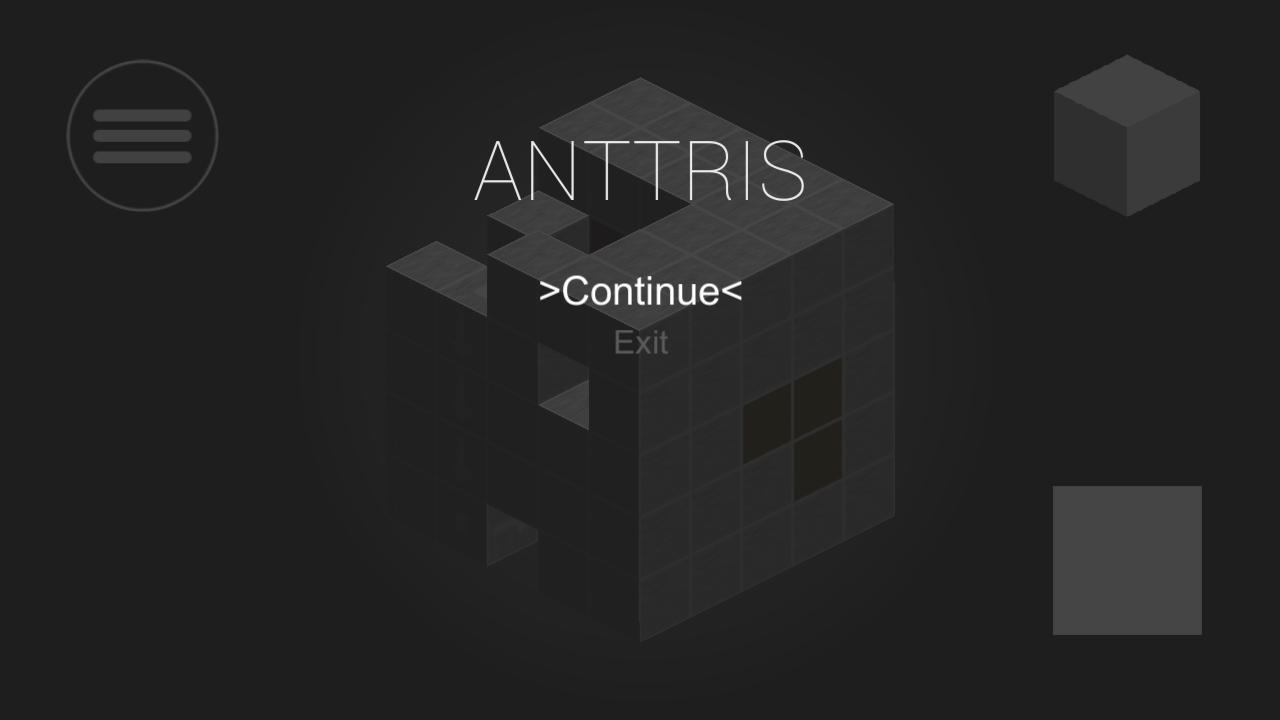
\includegraphics[width=4in]{GamePauseUI.png}
        \caption{Paused Game UI. This leads back to the Game UI or to the Play Menu UI. }
    \end{figure}
    \begin{figure}[H]
        \centering
        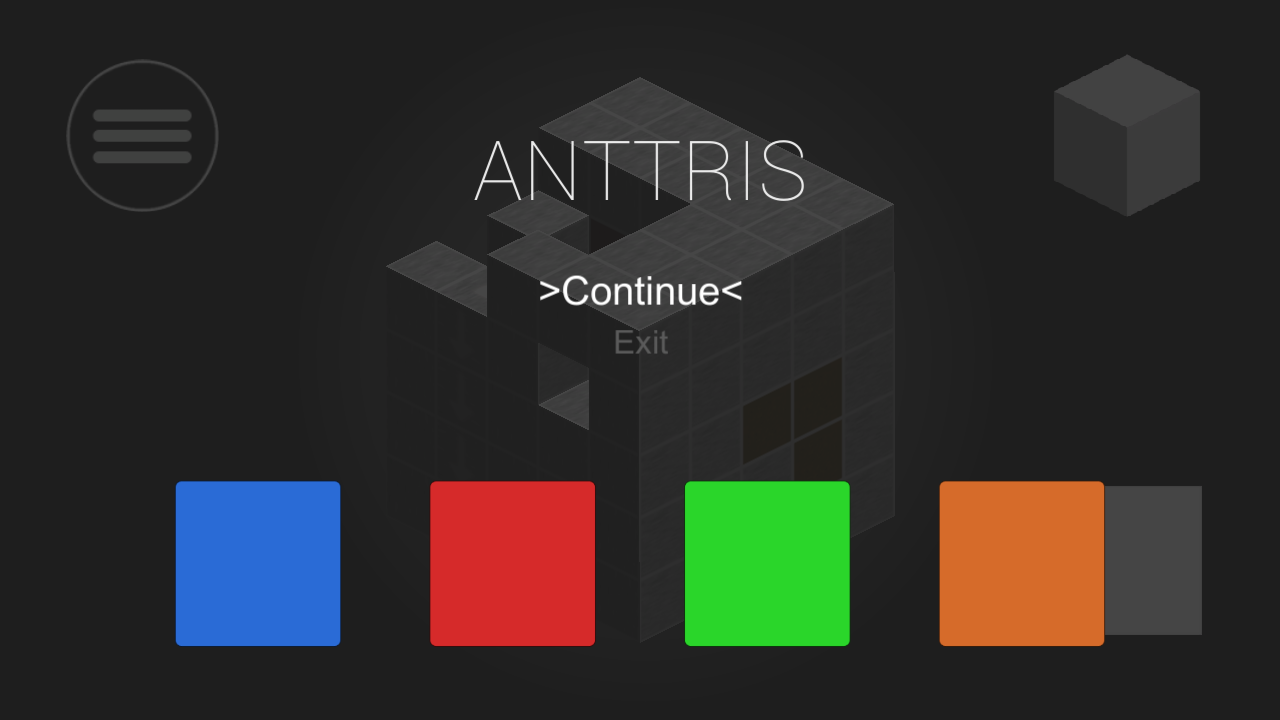
\includegraphics[width=4in]{EditorMenuUI.png}
        \caption{Editor Menu UI. This leads back to the Editor UI or to the Main Menu. Colored squares are placeholders for different kinds of blocks. }
    \end{figure}

% validation and criteria
\section{Validation and Criteria}\label{validation-BC}
 Since we are crating an interactive puzzle game, we will be using the Black Box Testing method in order to test all the buttons, features, and interactions with the puzzle to make sure that all of the functions preform properly. 
 Testing these functions from a user perspective versus a coding perspective is very important since our game will be interacting with multiple blocks and functions of the game at one time. 
 After we complete the user end, we will use the White Box Testing method in order to test the code and pass parameters to each of the functions to ensure that our connections between players and the code itself is working properly. 
 We will know that we have satisfied a use case, when we know that each of the features and interactions between the different actors work properly.
% appendices
\section{Appendices}

\subsection{Project Status}\label{status-ST}

Much progress has been made. We have a working Javascript prototype, a
workable timeline for Scrum, and we have begun our first sprint. The
primary objective of this first sprint is to convert the prototype
into a project for the Godot game engine \cite{godot:gameengine}.

Currently, we plan to have four sprints of two weeks duration each,
with weekends acting as slack days. Due to scheduling, the first
sprint is slightly longer than two weeks, so we plan to do more to
offset the projected downtime during spring break. Sean has taken on the job of coordinating the team as Scrum Master.

Our team also has solid organization and collaboration thanks to various tools, including Github for our git repositories \cite{github:site}, Zenhub for integrated Agile project management in Github \cite{zenhub:site}, Slack for team collaboration \cite{slack:site}, and Travis CI for continuous integration \cite{travis:site}.

\begin{table}[h]
\centering
\begin{tabular}{|l|l|l|l|l|l|}
\hline
 & {\bf Sprint 1} & {\bf Sprint 2} & {\bf Sprint 3} & {\bf Sprint 4} & {\bf Sprint 5} \\ \hline
{\bf Date} & 2/18 - 3/6 & 3/9 - 3/21 & 3/23 - 4/3 & 4/6 - 4/17 & 4/21 - end \\ \hline
{\bf Goals} & Prototype & Get game working & Polish game & \specialcell{Advanced\\features} & \specialcell{Advanced\\features} \\ \hline
{\bf Issues} & None & Spring Break! & \specialcell{Deficiencies\\in design} & None & None \\ \hline
 &  &  &  &  &  \\ \hline
\end{tabular}
\caption{Scrum Timeline}
\label{timeline}
\end{table}

%\clearpage
\subsection{Task Assignments by Team Member}\label{assignments}
We have also assigned ourselves various tasks involved in the completion of the project. Included below is a table denoting our current assignments.

    \begin{figure}[H]
        \centering
        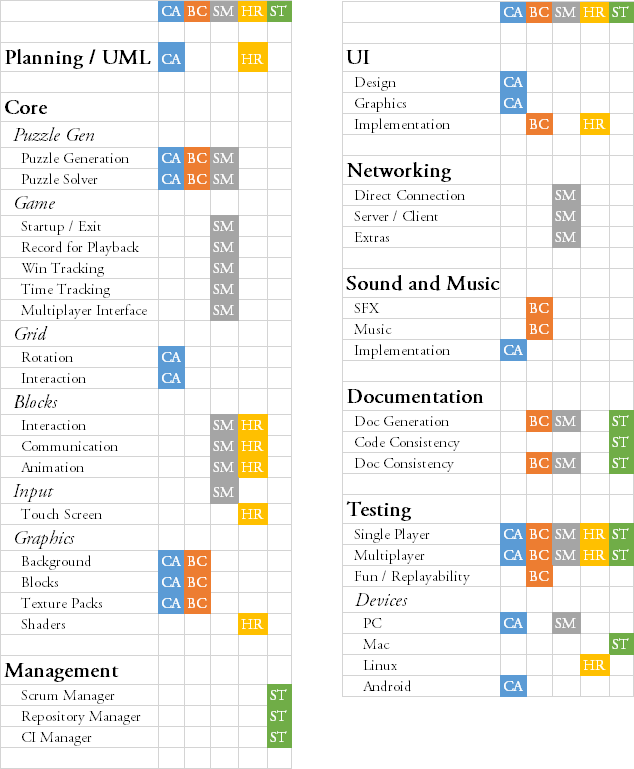
\includegraphics[width=5in]{Assignments.png}
        \caption{Current team member assignments. This is subject to change.}
    \end{figure}

\bibliographystyle{acm}
\bibliography{team5-requirements-spec}
\end{document}








